\documentclass[12pt]{article}

\usepackage{sbc-template}

\usepackage{graphicx,url}

\usepackage[brazil]{babel}
%\usepackage[latin1]{inputenc}
\usepackage[utf8]{inputenc}
% UTF-8 encoding is recommended by ShareLaTex


\sloppy

\title{Lock-o-tron}

\author{Rafael Sá Menezes\inst{1}, Rodrigo dos Santos Tavares\inst{1},
Felipe Leite Lobo\inst{1},\\Herbert Rocha\inst{1}, Thais Oliveira Almeida\inst{1} }


\address{Departamento de Ciência da Computação -- Centro de Ciência e Tecnologia
  \\Universidade Federal de Roraima (UFRR)\\
  Boa Vista -- RR -- Brazil
  \email{\{rafa.sa, rodrigo.tavares, felipe.lobo, herbert.rocha,}
  \email{thais.oliveira\}@ufrr.br}
}

\begin{document}

\maketitle

\begin{abstract}
    This paper describes the main features of Lock-o-tron, a security system
    based on facial recognition, while presenting its algorithms, modules,
    configuration, connections, libraries used and future works. The algorithms
    mentioned are Fisherfaces (for facial recognition) and fifo (for real-time
    scheduling). OpenCV was used as the facial recognition engine, and an Intel
    Galileo for controlling a motion sensor and an electric lock. At last, the
    system was able to achieve its goal.

\end{abstract}

\begin{resumo}
    Este artigo descreve as principais características do Lock-o-tron, um
    sistema de segurança com reconhecimento facial, abordando seus algoritmos,
    módulos, disposição, conexões, bibliotecas utilizadas e possibilidades de
    trabalhos futuros. Os algoritmos descritos são \textit{Fisherfaces} (para
    reconhecimento facial) e o de fifo (para escalonamento em tempo-real).
    Foi utilizado OpenCV para fazer o reconhecimento dos rostos, e um Intel
    Galileo para controle de um sensor de presença e de uma fechadura elétrica.
    Ao final, concluímos que fomos capazes de atender a tarefa proposta.
\end{resumo}


\section{Introdução}
    O Lock-o-tron é um projeto interdisciplinar que, unindo os conceitos de
    diversos campos da Computação, realiza o reconhecimento facial de pessoas. O
    sistema conta com: Um servidor, um Intel Galileo, um Yocto Linux configurado
    para \textit{soft-realtime}, diversos sensores, diversos atuadores, uma
    interface Web para administração e um aplicativo Android para controle.

    Este trabalho irá descrever as principais características do sistema, assim
    o leitor poderá entender melhor sobre o funcionamento do sistema como um
    todo.

%\section{Lock-o-tron}

\section{Dispositivos}
    O sistema é dividido em duas partes principais: O Galileo, responsável por
    controlar, e o servidor, responsável por administrar. A figura \ref{fig:bigpicture}
    contém o \textit{Big Picture} do Lock-o-tron.

   \begin{figure}[ht]
		\centering
		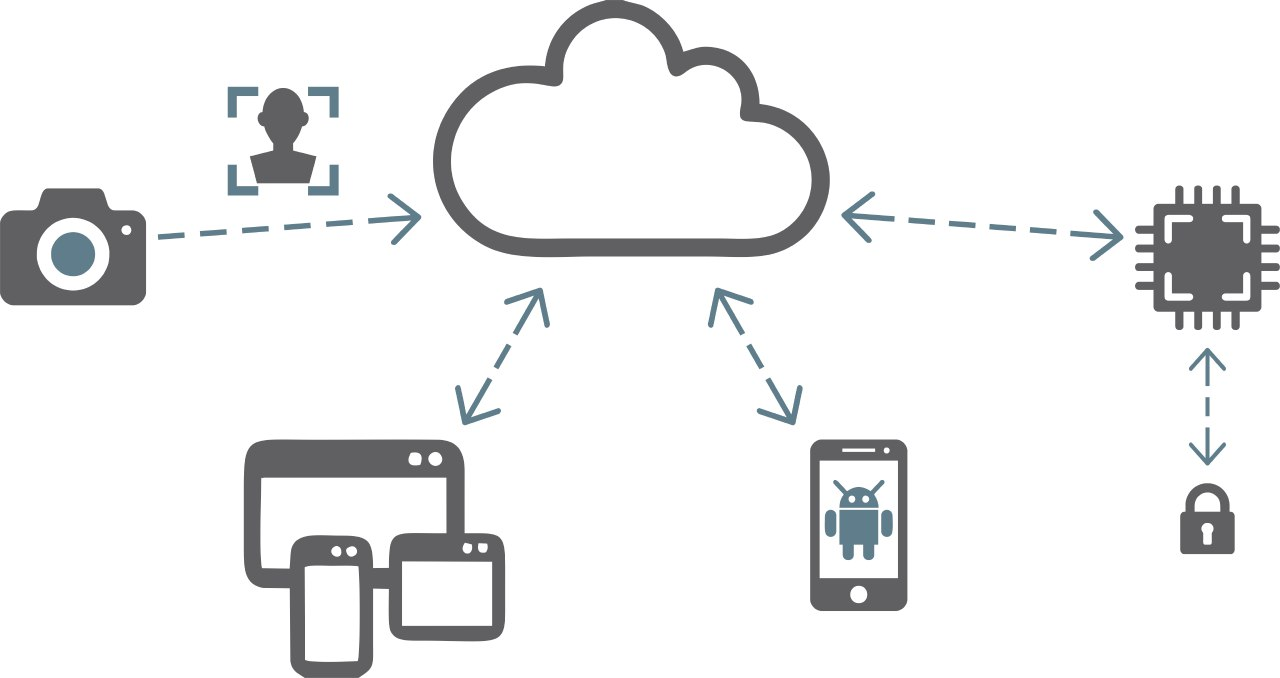
\includegraphics[width=.5\textwidth]{big-picture}
		\caption{Big Picture}
		\label{fig:bigpicture}
	\end{figure}


\subsection{Galileo}
    No Galileo conectamos:
    \begin{description}
        \item[Sensor de Presença:] Responsável por detectar se existe alguma
        pessoa no local para que o sistema saiba quando deve iniciar o
        reconhecimento facial;
        \item[Fechadura elétrica:] A fechadura é o atuador final do sistema,
        sendo ativada para abrir a porta.
    \end{description}

    A figura~\ref{fig:schema} mostra o esquema do circuito em um Galileo. Na
    aplicação real, porém, o LED seria substituído por uma fechadura elétrica,
    sem muitas alterações no circuito.

   \begin{figure}[ht]
		\centering
		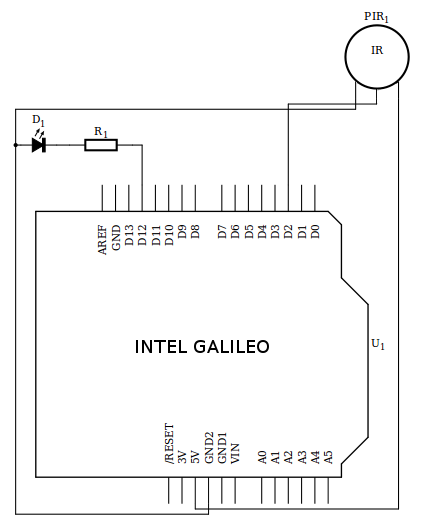
\includegraphics[width=.5\textwidth]{schematics}
		\caption{Esquema do circuito do Galileo}
		\label{fig:schema}
	\end{figure}

\subsection{Servidor}
    No Servidor conectamos:
    \begin{description}
        \item[Câmera:] A câmera obtém os frames e os salva no servidor.
    \end{description}

\subsection{Orçamento}
% Salário esperado: R$2000,00 => R$/h = 17
	O orçamento foi baseado em que cada programador receberia R\$2000,00 mensais
	(sendo 20 dias úteis), trabalhando 6 horas por dia. O projeto levou em torno
	de 30 dias para ser desenvolvido. A tabela \ref{orcamento} mostra o orçamento
	do projeto

	\begin{table}[]
	\centering
	\caption{Orçamento}
	\label{orcamento}
	\begin{tabular}{ll}
	\textbf{Produto}         & \textbf{Valor} \\
	Intel Galileo            & R\$ 499,90     \\
	Sensor de presença       & R\$ 18,90      \\
	Câmera                   & R\$ 200,00     \\
	Fechadura elétrica       & R\$ 159,00     \\
	Implementaçao do Sistema & R\$ 6.120,00   \\
	\textbf{Total:}          & R\$ 6.997,80   \\
                         &
	\end{tabular}
	\end{table}


\section{Comunicação interna}
    Para comunicação do sistema foram utilizados: um servidor UDP, um
    \textit{web service} e uma interface Web.

\subsection{Servidor UDP}
    Esse servidor UDP, que é executado no Galileo, é responsável pela interação
    de outros ambientes com o Galileo. Através destas mensagens UDP é possível
    abrir a porta e solicitar atualizações.
    A prioridade do servidor UDP é a mais alta no Galileo, então, sempre que
    alguém enviar uma mensagem, os outros processos serão interrompidos para que
    a ação pedida seja executada. A figura \ref{fig:petri-udp} mostra a rede de
    Petri que representa as computações do servidor UDP.

    \begin{figure}[ht]
		\centering
		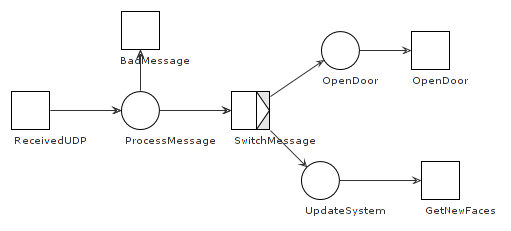
\includegraphics[width=.7\textwidth]{petri-udp}
		\caption{Rede de Petri do servidor UDP}
		\label{fig:petri-udp}
	\end{figure}

\subsection{Web Service}
    O \textit{web service}, executado no servidor, foi desenvolvido em PHP e é responsável pela interação de todos os ambientes entre si. As suas funções são:
    \begin{itemize}
        \item Enviar frames para o Galileo;
        \item Enviar atualizações para o Galileo;
        \item Enviar requisições UDP de abrir porta para o Galileo;
        \item Enviar requisições UDP de atualizar para o Galileo;
        \item Alterações no banco de dados (utilizando PDO);
        \item Requisições do banco de dados (utilizando PDO).
    \end{itemize}

\subsection{Interface Web}
    A interface Web, executada no servidor, ficou responsável por ser um meio
    multiplataforma para modificar o banco de dados. Foi utilizado o \textit{framework Material Design Lite} para CSS.

\section{Reconhecimento Facial}
% tamanho fisherface: 60 frames 4 pessoas = 534,5kb
% tamanho eigenface: 60 frames 4 pessoas = 31,4MB
    Para o reconhecimento facial, foram utilizados os algoritmos de	\textit{Fisherfaces} e \textit{Eigenfaces}. Para 4 pessoas, obtendo 60 frames
    o \textit{Fisherfaces} ocupou $534,5$KB's, já o \textit{Eigenfaces} ocupou
    $31,4$MB's. Por se tratar de um sistema embarcado com espaço limitado, o
    algoritmo de \textit{Fisherfaces} foi escolhido como definitivo.
    O Galileo obtém o frame do servidor (um frame já pré-processado) e atribui
    um ID a esse frame. Caso o ID seja 255, o frame é considerado como sendo de
    ninguém conhecido, caso contrário, é enviada uma requisição ao
    \textit{web service} para descobrir se a pessoa está autorizada a entrar
    naquele horário. Caso ela esteja autorizada, a fechadura abre.

    Os frames são pré-processados com as seguintes etapas:
    \begin{enumerate}
        \item Aplica-se uma conversão para tons de cinza;
        \item Aplica-se uma equalização do histograma no frame;
        \item Procura-se os dois olhos da imagem, continua apenas se encontrar;
        \item Rotaciona-se o frame para os olhos ficarem alinhados no eixo x;
        \item Aplica-se uma equalização do histograma nos lados direito e
        esquerdo do rosto;
        \item Aplica-se o filtro de suavização;
        \item Aplica-se uma máscara elíptica para remoção do pescoço.
    \end{enumerate}
     Tudo isso para normalizar todos os frames e facilitar o reconhecimento
     facial.

     O treinamento é feito ao pegar 60 frames pré-processados (da mesma pessoa)
     e associa-se essa pessoa a um ID (o mesmo utilizado no banco de dados),
     então é utilizado o algoritmo de \textit{Fisherfaces} (que já vem
     implementado no opencv2) para o treinamento e é gerado um xml (treinado)
     com esses dados. Posteriormente, o Galileo obtém esse XML e aplica o
     algoritmo de \textit{Fisherfaces} em um frame pré-processado. A figura
     \ref{fig:petri-reconhecimento} ilustra a rede de Petri das computações
     de reconhecimento facial no Galileo.

     \begin{figure}[ht]
		\centering
		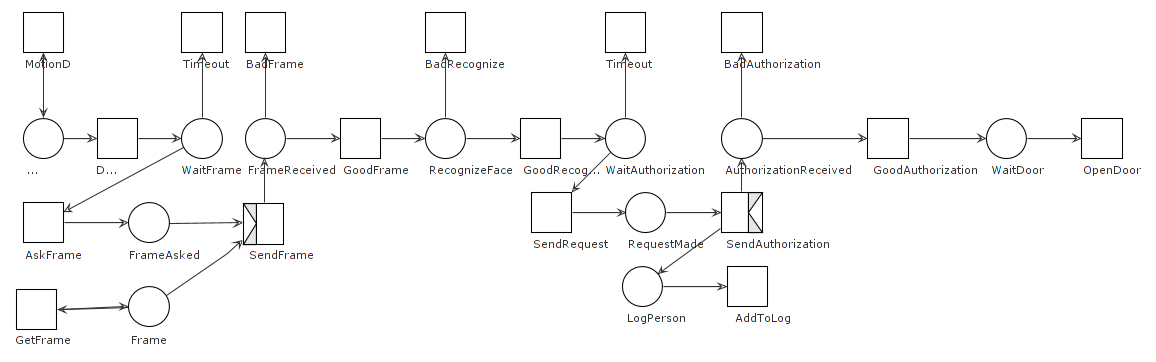
\includegraphics[width=1\textwidth]{petri-reconhecimento.png}
		\caption{Rede de Petri do Reconhecimento}
		\label{fig:petri-reconhecimento}
	\end{figure}

\section{Sistema Operacional}
    O sistema operacional utilizado no servidor é um GNU/Linux genérico, já no
    Galileo, é utilizado o Yocto Linux com o kernel configurado para
    \textit{preempt}.

\subsection{Yocto Linux}
    O Yocto Linux é uma distribuição de Linux desenvolvida especificamente para
    sistemas embarcados. Para o Galileo, a Intel disponibiliza uma
     \textit{recipe} específica, que dá suporte à placa e aos seus pinos.

    Essa \textit{recipe} adiciona uma biblioteca chamada \textit{mraa},
    que facilita a interação das portas, removendo a necessidade de se acessar
    as GPIO diretamente.

\subsection{PREEMPT - Tempo Real}
    O projeto utiliza um algoritmo de \textit{soft-realtime}, já presente no
    Linux (configurado com \textit{preempt}), o \textit{fifo}. Este algoritmo tem
    prioridade sobre qualquer outra forma de escalonamento presente no sistema
    e executa o escalonamento da seguinte forma:
    \begin{itemize}
        \item Procura-se processo com maior prioridade FIFO (0 - menor, 100 -
        maior);
        \item Executa-se o processo até ele terminar ou receber uma mensagem de
        \textit{yield};
    \end{itemize}

    No Lock-o-tron, foi definido o servidor UDP com uma prioridade de 60 e o
    reconhecimento facial com prioridade 40. Todos os demais processos do
    sistema operacional não estão incluídos na tabela de tempo-real, então são
    os últimos a serem escalonados na tabela.

    Por ser um algoritmo de tempo-real estático, o \textit{fifo} não consegue
    garantir que irá cumprir todos os \textit{deadlines}, mas, os resultados
    obtidos apenas com ele foram muito positivos.

\section{Aplicativo Android}
    O aplicativo utiliza o \textit{web service} para comunicação com o Galileo e obtenção do histórico. Conta com os seguintes módulos:
    \begin{description}
        \item[Histórico:] Menu onde é possível visualizar os últimos usuários que
        tentaram entrar.
        \item[Panic Button:] Botão de emergência, quando pressionado a porta
        abre;
        \item[Update Button:] Botão para o Galileo atualizar seu arquivo de
        treinamento;
        \item[Estatísticas:] Menu onde é possível ver diversas informações sobre
        o uso do sistema.
    \end{description}

    As figura~\ref{fig:android} mostra as telas do aplicativo.

    \begin{figure}[!h]
		\centering
		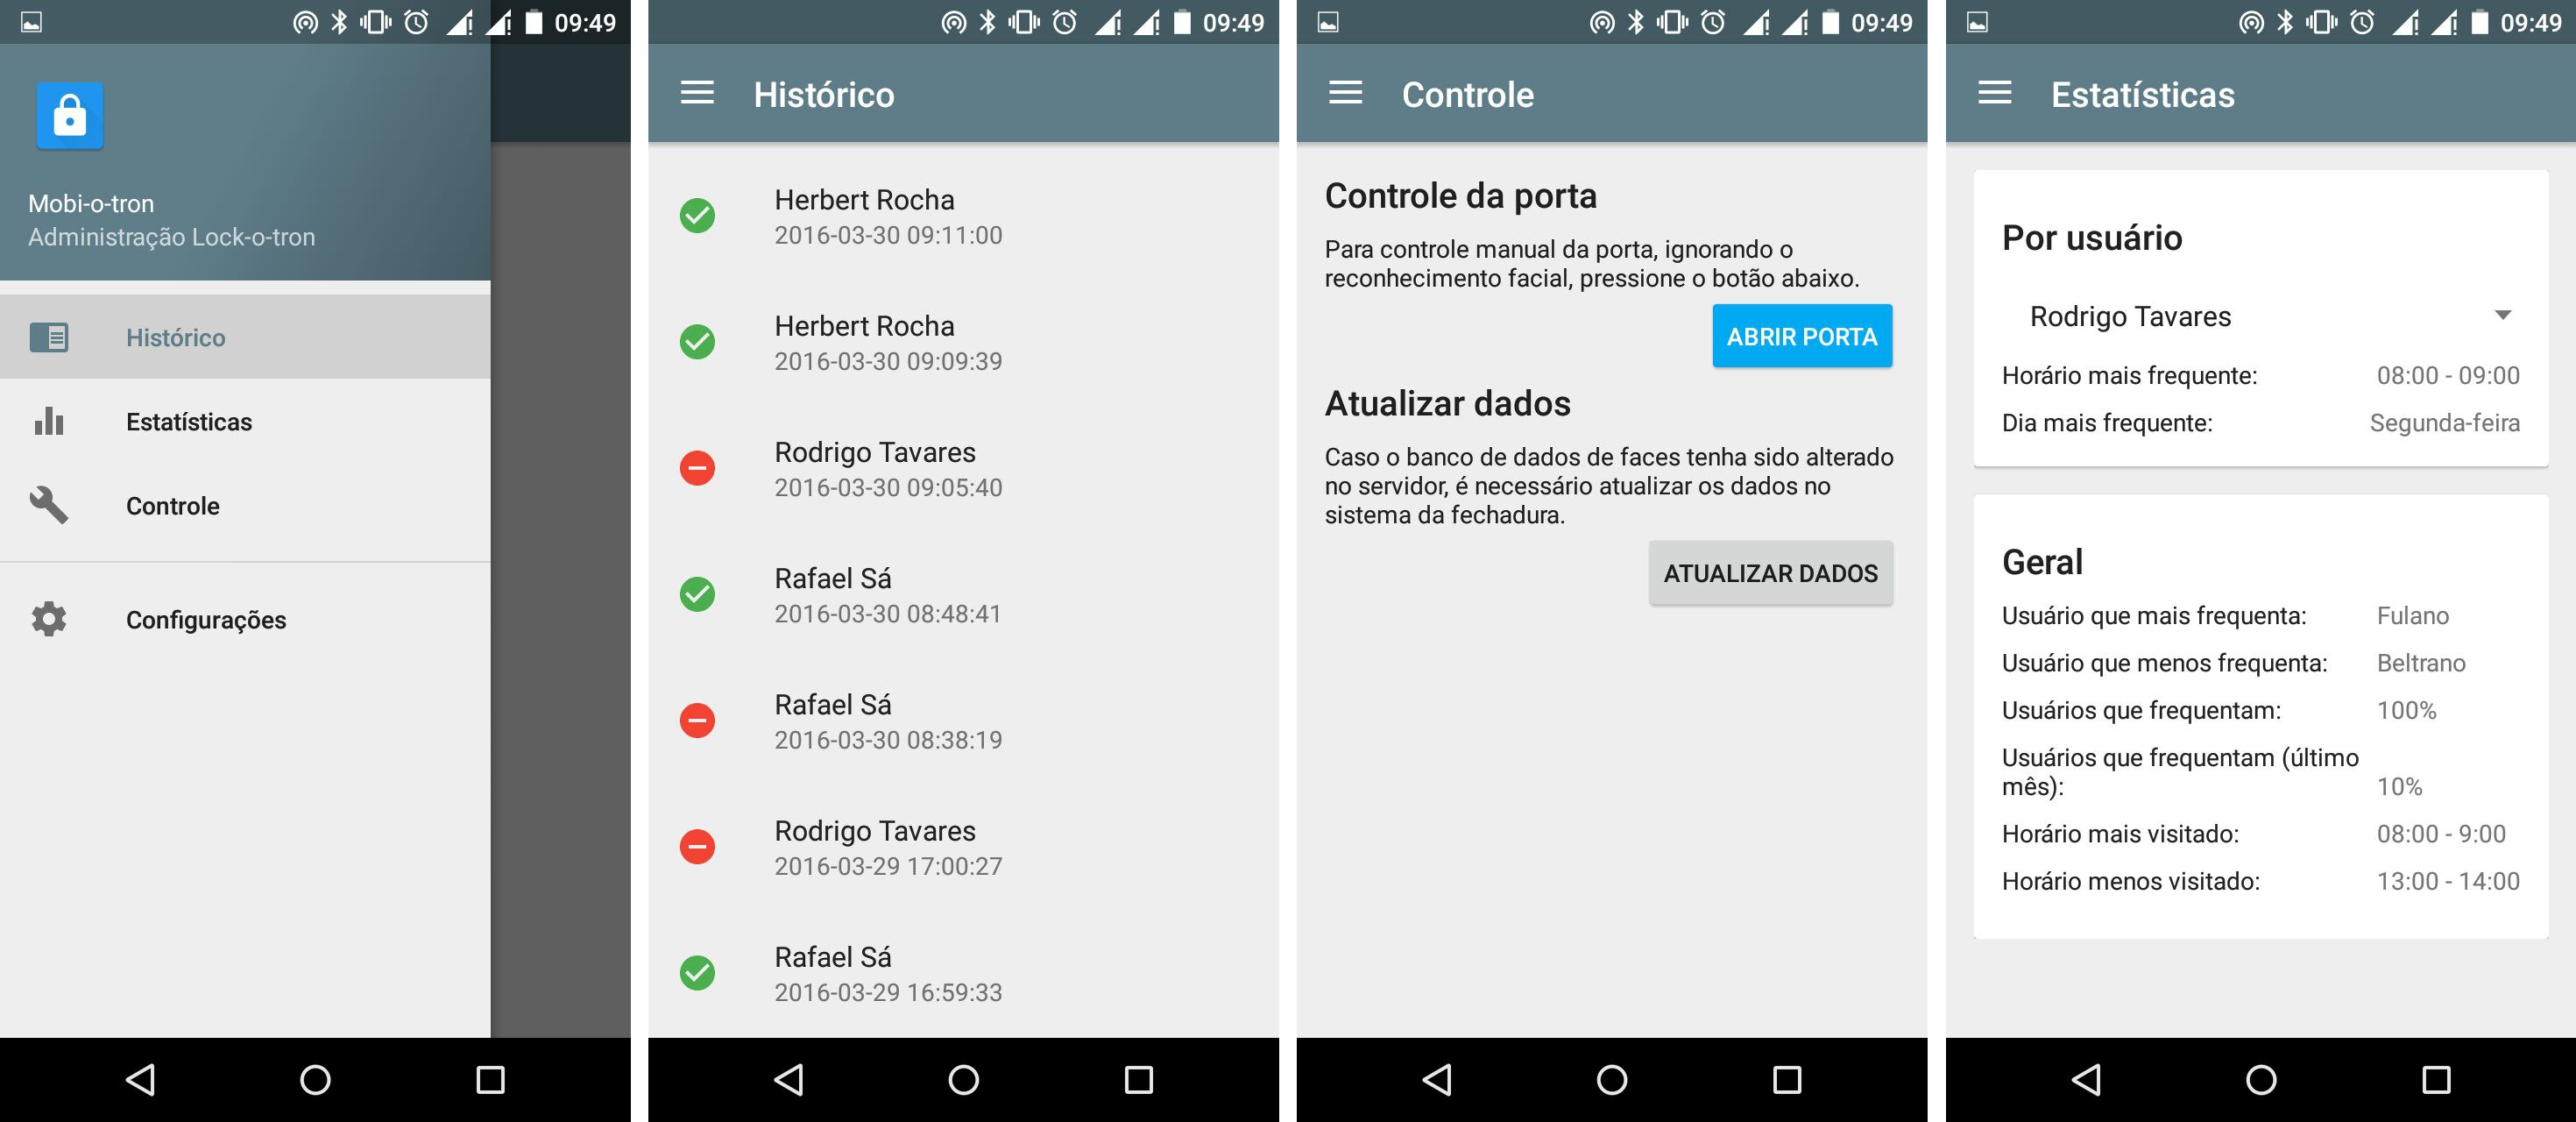
\includegraphics[width=1\textwidth]{android}
		\caption{Telas do aplicativo}
		\label{fig:android}
	\end{figure}


\section{Banco de Dados}
	O sistema utilizou um banco de dados SQL, o \textit{MySQL}, para armazenamento dos dados. A figura~\ref{fig:ent-rel} mostra o diagrama de entidade-relacionamento. Foi utilizado as seguintes tabelas:

		\begin{description}
			\item [usuario:] Utilizada para armazenar o usuários do sistema;
			\item [historico:] Utilizada para armazenar os \textit{logs} de quem tentou entrar (armazenando se obteve acesso ou não) e qual a data/hora;
			\item [autorizacao:] Utilizada para armazenar quais horários e dias os usuários estão autorizados a entrar.
		\end{description}

		\begin{figure}[!h]
		\centering
		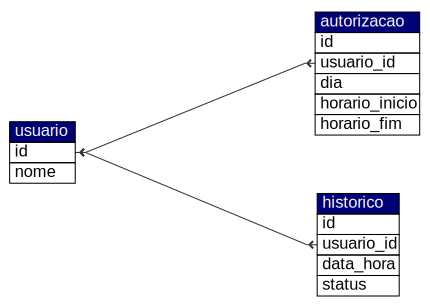
\includegraphics[width=0.6\textwidth]{bd-der}
		\caption{Diagrama entidade-relacionamento}
		\label{fig:ent-rel}
	\end{figure}

\section{Trabalhos Futuros}
    O Lock-o-tron abre portas para diversas possibilidades de expansão:
    \begin{itemize}
        \item Melhorar o algoritmo de reconhecimento;
        \item Adicionar novos níveis de segurança;
        \item Verificar número de pessoas que estão entrando em conjunto;
        \item Automação da sala adaptável às preferências do usuário reconhecido;
        \item Um sistema para identificação de padrões de comportamento estranhos.
    \end{itemize}

\section{Conclusão}
    Neste artigo foi apresentado as principais característica do Lock-o-tron, um
    sistema de segurança com reconhecimento facial, descrevendo seus algoritmos,
    módulos, disposição e bibliotecas utilizadas.

    No final, o sistema criado é capaz de executar a tarefa proposta com certa
    precisão (ainda sendo ajustada), e o escalonador garante que por mais
    sobrecarregado o Galileo esteja, as tarefas sempre serão executados em tempo
    hábil.

% \bibliographystyle{sbc}
% \bibliography{relatorio}




\end{document}
